% Generated by ASTES Journal Editorial Team
\documentclass{article} %%% use \documentstyle for old LaTeX compilers
\usepackage{geometry}
 \geometry{
 a4paper,
 total={170mm,257mm},
 left=20mm,
 top=20mm,
 }

\usepackage[english]{babel} %%% 'french', 'german', 'spanish', 'danish', etc.
\usepackage{amssymb}
\usepackage{amsmath}
\usepackage{multirow}
\usepackage{txfonts}
\usepackage{multicol}
\usepackage{booktabs}
\usepackage{mathdots}
\usepackage[classicReIm]{kpfonts}
\usepackage{graphicx} %%% use 'pdftex' instead of 'dvips' for PDF output
\usepackage{fancyhdr}
\usepackage{hyperref}
\usepackage{float}
\usepackage{microtype}
\usepackage{subcaption}
\usepackage[justification=centering]{caption}
\pagestyle{fancy}



%Paste this code in page 1
\fancyhead{}
\fancyhead[C]{ }
\renewcommand{\headrulewidth}{0pt }
\fancyfoot{}
\fancyfoot[L]{\href{http://www.astesj.com}{www.astesj.com}}
\fancyfoot[R]{\thepage}
%%%%%%%%%%%%%%%%%%%%%

% You can include more LaTeX packages here 

\makeatletter
\def\@xfootnote[#1]{%
  \protected@xdef\@thefnmark{#1}%
  \@footnotemark\@footnotetext}
\makeatother


\begin{document}

%\selectlanguage{english} %%% remove comment delimiter ('%') and select language if required



\begin{tabular}{p{1in}p{3.8in}p{1.2in}}  
\hspace{-1cm}
\noindent
\begin{tabular}{c}  
\includegraphics[width=2.9cm]{images/ASTES_Logo.jpg}\end{tabular} 	& \centering \textit{Advances in Science, Technology and Engineering Systems Journal \newline Vol. 3, No. 3, XX-YY (2018)} \\   \href{http://www.astesj.com}{www.astesj.com}  
	& \vspace{-0.6cm}  \rule{1.2in}{0.5pt} \vspace{-0.2cm} \newline \centering  \textbf{ ASTES Journal \newline ISSN: 2415-6698} \newline \rule{1.2in}{0.5pt} 
\end{tabular}


\vspace{1.8cm}






\noindent  \textbf{ \LARGE{\setlength\itemsep{0pt}Automatize landmarks setting on Species morphometry using Deep Neural Networks}}

\vspace{0.2cm}

Van-Linh Le\footnote[*]{Corresponding Author Name, Address, Contact No \& Email}${}^{,1,2}$, Marie Beurton-Aimar${}^{1}$, Akka Zemmari${}^{1}$, Nicolas Parisey${}^{3}$

\vspace{0.2cm}
 \textit{${}^{1}$LaBRI-CNRS 5800, University of Bordeaux, 33400, France}

\vspace{0.2cm}
\textit{${}^{2}$ITDLU, Dalat University, 670000, Vietnam}

\vspace{0.2cm}
 \textit{${}^{3}$IGEPP, INRA-1349, 35653, France}

\vspace{0.3cm}

\begin{tabular}{p{1.7in} p{0.1in} p{4.1in} }
A R T I C L E  I N F O &  & A B S T R A C T \\ 
 \cline{1-1}  \cline{3-3} \setlength\itemsep{0pt} \vspace{-0.1cm}
\textit{Article history:\newline Received: \newline Accepted:  \newline Online:  \rule{1.78in}{0.5pt} Keywords: \newline Landmarks\newline Morphometry setting\newline Deep learning\newline Convolutional neural networks} \newline \newline  & & \vspace{-0.1cm} \textit{
Morphometry landmarks are known as one of the
approaches to analyze the characteristics of organisms. Finding
landmarks setting can give to biologists a comprehensive description of the organism. In this study, we propose a convolutional
neural network (CNN) to predict the landmarks on biological's species.
The network is designed as a combination of the ``elementary blocks".
After training with a set of manually landmarks dataset, 
it has been used to predict the morphometric landmarks on biological images automatically.
The network has been checked by applying two scenarios: training from scratch and fine-tuning.
The predicted landmarks have been evaluated by comparing with the coordinates of manual landmarks which have been provided by the biologists.
 The network model is implemented by Python on
Lasagne framework. }\\
 \cline{1-1}  \cline{3-3}
\end{tabular}


\vspace{0.3cm}

\begin{multicols}{2}



\section{ Introduction}
Morphometry analysis refers to measure the topography of an object, for example, its shape and its size. Biologists work with several parameters from organisms such as lengths, widths, masses, angles,... to analyze the interactions between environment and organisms development. Besides the traditional information, landmarks (or points of interest in the image) are known as one of the characteristics to analyze the shape. Instead of collecting all information, the shape is determined by a finite set of points, called landmarks. Landmarks store important information about the shape of the object, \textit{for example}, the corners of the human mouth are a kind of landmarks. Mostly, the landmarks are along the outline of the object but in some special cases, it could be defined inside the anatomical part, \textit{i.e} the landmarks on Drosophila wings are the intersection of veins on fly wings, but the landmarks on pronotum can be located at the shape edge or inside the pronotum. In our study, the morphometric landmarks are specific points defined by biologists. They are used in many biological studyings. Currently, the landmarks are set manually by the entomologist, the operation are time-consuming and difficult to reproduce when the operators change. Therefore, a method that gives automatic location of landmarks could have a lot of interest.

In this study, we have used a dataset including the images of collecting from $293$ beetles in Brittany lands. All the images are presented in RGB color with two dimensions. For each beetle, the biologists took images of five parts: \textit{left and right mandibles, head, body, and pronotum} (Fig.\ref{fig1}). For each part, a set of manual landmarks has been positioned by an entomologist.

In the concept of automatically landmarks setting, image processing is usually the first choice to apply. This is a process that we apply a set of algorithms (in image processing) to extract and to analyse the object of interest. In which, segmentation is most often the first and the most important step. This task remains a bottleneck to compute features of an image. In some cases, the object of interest is easy to extract and can be analyzed with the help of a lot of very well-known image analysis procedures. Like previous study \cite{.}, we have analyzed two parts beetle mandibles (Fig.\ref{figsub01} and Fig.\ref{figsub02}). These parts are pretty easy to segment (enough good quality for our goals). In that work, we have applied a set of algorithms based on the combination of principal component analysis \cite{shlens2014tutorial} and SIFT descriptor \cite{lowe2004distinctive}. 
Unfortunately, this method is irrelevant with the case of the images that are not precise or difficult to segment, \textit{i.e.} pronotum images. So, the remain question of how to predict the landmarks on the images like the pronotum images? This is the reason why we have turned to a way of analyzing images without need for a segmentation step. So, the next step has been to work with the prontoum images (Fig.\ref{figsub05}). For each pronotum image, a set of 8 manual landmarks have been set by the biologists (Fig.\ref{.}). They are considered as the ground truth to evaluate the predicted landmarks by our method.

\begin{figure}[H]
    \centering
    \begin{subfigure}[t]{0.23\textwidth}
        \centering
        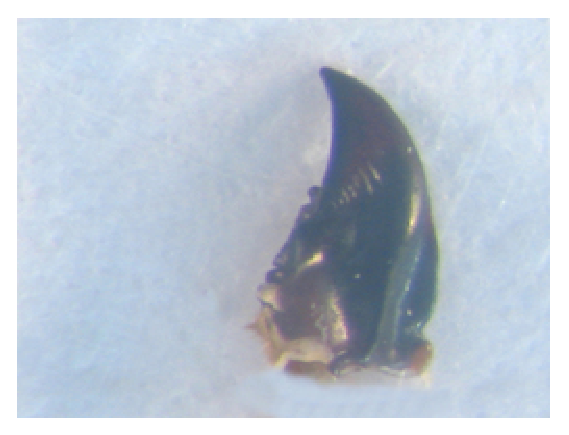
\includegraphics[height=1in]{images/md19.eps}
        \caption{Right mandible}
        \label{figsub01}
    \end{subfigure}%
    ~ 
    \begin{subfigure}[t]{0.23\textwidth}
        \centering
        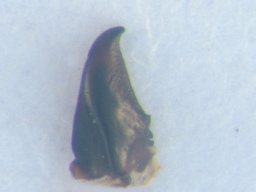
\includegraphics[height=1in]{images/mg019.JPG}
        \caption{Left mandible }
        \label{figsub02}
    \end{subfigure}~\\
    \begin{subfigure}[t]{0.23\textwidth}
        \centering
        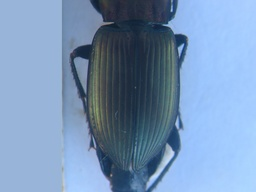
\includegraphics[height=1in]{images/elytre107.JPG}
        \caption{Elytra}
        \label{figsub03}
    \end{subfigure}%
    ~ 
    \begin{subfigure}[t]{0.23\textwidth}
        \centering
        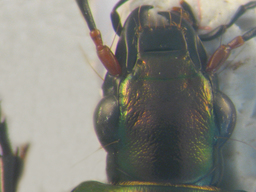
\includegraphics[height=1in]{images/tete081.JPG}
        \caption{Head }
        \label{figsub04}
    \end{subfigure}~\\
    \begin{subfigure}[t]{0.23\textwidth}
        \centering
        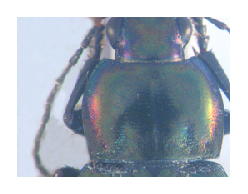
\includegraphics[height=1in]{images/prono60.eps}
        \caption{Pronotum/thorax }
        \label{figsub05}
    \end{subfigure}
    \caption{The anatomical parts of beetle}
    \label{fig1}
\end{figure}

To achieve the landmarks prediction, this work introduces a method for this automatic detection of the landmarks on pronotum images. The main idea consists on design and train of a CNN \cite{lecun2010convolutional} with a set of manual landmarks. In the first stage, the network has been trained from scratch on the dataset of pronotum images from the first model. In the second step, the training has been modified to improve the quality of prediction by including the fine-tuning\cite{.} step. The network has been implemented by using Python on Lasagne library \cite{.}.

\begin{figure}[H]
	\centering
	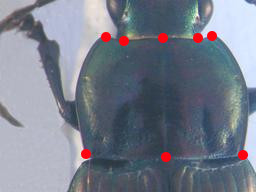
\includegraphics[height=1.6in]{images/pronotum.jpg}
	\caption{A pronotum image with its eight manual landmarks}
	\label{figconvarc}
\end{figure}

The rests of the article is organized as follows. In the next sections, we first give a briefly overview of the related works on automatically landmarking. We then shortly present an overview about CNN. After that, in Section X1, we describe the architecture of the proposed network and its parameters also. The dataset augmentation processes are presented in Section X2. In Section X2, we give the first results of the model, then we present the step of fine-tuning to improve the result. Finally, we conclude the article with a discussion of future works in Section X3.

\section{Related works}
A landmark is a specific point that may contain useful information. For example, the tip of the nose or the corners of the mouth are landmarks on human face \cite{sun2013deep}. Under image processing point of view, when we want to extract the feature from the image, we can consider two kinds of cases: the object of interest can be segmented or not. Setting landmarks can not be achieved in the same way depending on which situation we are. When segmentation can be applied, Lowe et al. \cite{lowe2004distinctive} have proposed SIFT method to find the corresponding keypoints in the 2D images. From the detected keypoints, the method is able to match two images. Palaniswamy et al. \cite{palaniswamy2010automatic} have proposed a method based on probabilistic Hough Transform to automatically locate the landmarks in digital images of Drosophila wings. In previous work \cite{le2017maelab}, we have proposed a method which have been extended from Palaniswamy's method, to determine landmarks on mandibles of beetles. The mandibles of beetle have the simple shape and easy to segment. We have obtained good enough results about determining the landmarks automatically on mandibles. Unfortunately, after several tests, we have had to conclude that this way does not provide good results with the pronotum images because the pronotum segmentation has too many noises.

In recent years, deep learning is known as a solution for many task in different topics. In image analysis domain, using deep learning, namely CNN, to determine the landmarks on 2D images has achieved better results even if the images that can not segment. Yi Sun et al. \cite{sun2013deep} have proposed cascaded CNNs to predict the facial points of interest on the human face.
Zhanpeng Zhang et al. \cite{zhang2014facial} proposed a \textit{Tasks-Constrained Deep Convolutional Network} to optimize facial landmarks detection. Their model determines the facial landmarks with a set of related tasks such as head pose estimation, gender classification, age estimation, face recognition, or facial attribute inference. Cintas et al. \cite{cintas2016automatic} has introduced a network to predict the landmarks on human ears. After training, the network has the ability to predict 45 landmarks on human ears. In this way, we have applied CNN computing to work with pronotum landmarks.

\section{Convolutional neural networks}
Deep learning models are coming from the machine learning theory. They have been introduced in the middle of previous century for artificial intelligence applications but they encounter several problems to take real-world cases. Fortunately, the improvement of computing capacities both in memory size and computing time with GPU programming has opened the new perspective for deep learning. 

Deep learning allows computational model composed of multiple processing layers to learn representations of data with multiple levels of abstraction \cite{lecun2015deep}. Each layer extracts the representation of the input data from the previous layer and computes a new representation for the next layer. In the hierarchy of a model, higher layers of representation enlarge aspects of the input that is important for discrimination and suppress irrelevant variations. Each level of representations is corresponding to the different level of abstraction. During training, it uses gradient descent optimization method to update the learnable parameters via backpropagation. The development of deep learning opens promise results for well-known problems artificial intelligence on high dimensional data, therefore applicable to many domains: image recognition and classification \cite{krizhevsky2012imagenet,ciregan2012multi,szegedy2015going}, speech recognition \cite{mikolov2011strategies,hinton2012deep,sainath2013deep}, question answering \cite{bordes2014question}, language translation \cite{sutskever2014sequence} \cite{jean2014using}, and recognition \cite{li2015convolutional}\cite{tompson2014joint}.

A CNN consists of a number of connected layers. The layers of a CNN has neurons arranged in three dimensions: \textit{width, height, and depth} with learnable parameters. Fig. \ref{figconvarc} shows a classical example of CNN. It is a pipeline of usual layers: convolutional layers (CONV), pooling layers (POOLING), dropout layers (DROPOUT), and full-connected layers (FC).

\begin{figure}[H]
	\centerline{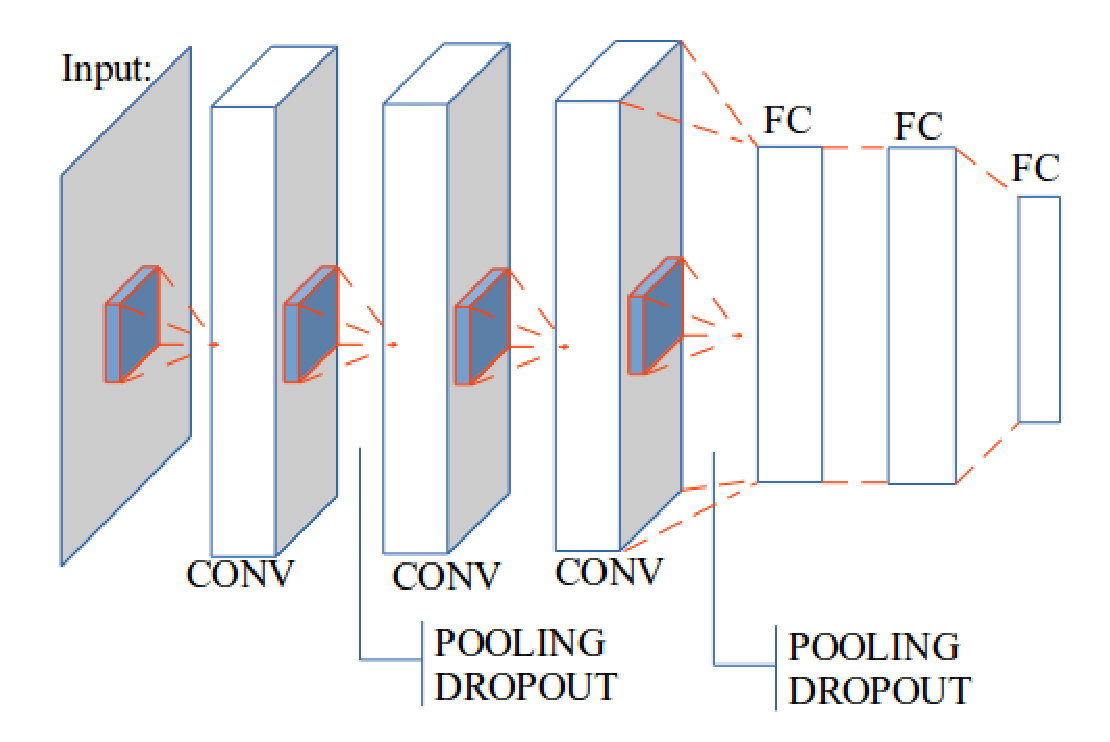
\includegraphics[height=1.8in]{images/convarc.eps}}
	\caption{An example of usual convolutional neural network}
	\label{figconvarc}
\end{figure}

A \textit{convolutional} layer computes a dot product between its weights and a small region in the input. At the output, the results of connected local regions are combined. Convolution layer uses a set of learnable filters as parameters. Each filter is small spatially but extends the depth of the input. \textit{Pooling} layer is used to down-sampling the input, to reduce the computational cost in remaining layers, and to control overfit. \textit{Dropout} layer refers to dropping out units in the network. Dropping a unit out means temporarily removing it from the network, along with all its incoming and outgoing connections. \textit{Full connected} layer refers to the output of the network. The number of outputs of the last full-connected layer are corresponding to the number of predicted values.

From the beginning of deep learning until now, many deep learning frameworks have been developed.
These frameworks help the users to design their application by re-using already proposed network architectures. Almost frameworks are open source. According to the written programming languages, the frameworks can be separated into two main groups: C++, \textit{such as Caffe, Deeplearning4j, Microsoft Cognitive Toolkit} and Python \textit{i.e Keras, Theano, PyTorch}. Another framework exists using more confidential languages as \textit{Lua}.

Theano \cite{theanoframework} is an open source framework developed by the machine learning group at the University of $Montr\acute{e}al$. It is a Python library that allows to define, to optimize and to evaluate mathematical expressions relating multi-dimensional arrays efficiently by using a Numpy package. Theano supports compilation on either CPU or GPU architectures. Lasagne \cite{lasagne} is a lightweight library in Theano. It allows to build and to train the neural networks. In this work, we have used Lasagne to implement the proposed neural network. Recently, Theano has been stopped to develop but its community is still large. The networks which have been designed by Theano are still useful and efficient in deep learning area.
\section{Application to landmarks identification}


\subsection{Maintaining the Integrity of the Specifications (Heading 2)}



The template is used to format your paper and style the text. All margins, column widths, line spaces, and text fonts are prescribed; please do not alter them. You may note peculiarities. For example, the head margin in this template measures proportionately more than is customary. This measurement and others are deliberate, using specifications that anticipate your paper as one part of the entire proceedings, and not as an independent document. Please do not revise any of the current designations.


\section{Prepare Your Paper before Styling}

Before you begin to format your paper, first write and save the content as a separate text file. Keep your text and graphic files separate until after the text has been formatted and styled. Do not use hard tabs, and limit use of hard returns to only one return at the end of a paragraph. Do not add any kind of pagination anywhere in the paper. Do not number text heads-the template will do that for you.

Finally, complete content and organizational editing before formatting. Please take note of the following items when proofreading spelling and grammar.


\subsection{Abbreviations and Acronyms}

Define abbreviations and acronyms the first time they are used in the text, even after they have been defined in the abstract. Do not use abbreviations in the title or heads unless they are unavoidable.



\begin{enumerate}
\item \textit{ }Use SI (MKS) as primary units. (SI units are encouraged.) English units may be used as secondary units (in parentheses). An exception would be the use of English units as identifiers in trade, such as ``3.5-inch disk drive''.

\item  Do not mix complete spellings and abbreviations of units: ``Wb/m2'' or ``webers per square meter'', not ``webers/m2''.  Spell out units when they appear in text: ``. . . a few henries'', not ``. . . a few H''.

\item  Use a zero before decimal points: ``0.25'', not ``.25''. Use ``cm3'', not ``cc''. (\textit{bullet list})
\end{enumerate}


\subsection{Equations}

The equations are an exception to the prescribed specifications of this template. You will need to determine whether or not your equation should be typed using either the Times New Roman or the Symbol font (please no other font). To create multi-leveled equations, it may be necessary to treat the equation as a graphic and insert it into the text after your paper is styled.
Number equations consecutively. Equation numbers, within parentheses, are to position flush right, as in (\ref{eq:1}), using a right tab stop. To make your equations more compact, you may use the solidus ( / ), the exp function, or appropriate exponents. Italicize all the symbols for quantities and variables, Use a long dash rather than a hyphen for a minus sign. Punctuate equations with commas or periods when they are part of a sentence, as in

\begin{equation}
\label{eq:1}
\alpha+\beta=\gamma
\end{equation}

Note that the equation is centered using a center tab stop. Be sure that the symbols in your equation have been defined before or immediately following the equation. Use ``(\ref{eq:1})'', not ``Eq. (\ref{eq:1})'' or ``equation (\ref{eq:1})'', except at the beginning of a sentence: ``Equation (\ref{eq:1}) is . . .''



%Paste this code in page 2
\fancyhead{}
\fancyhead[C]{\textit{S.S. Ahmad et al. / Advances in Science, Technology and Engineering Systems Journal Vol. 3, No. 1, XX-YY (2018)}}
\renewcommand{\headrulewidth}{1pt }
\fancyfoot{}
\fancyfoot[L]{\href{http://www.astesj.com}{www.astesj.com}}
\fancyfoot[R]{\thepage}
%%%%%%%%%%%%%%%%%%%%%

\subsection{Figures}

\begin{figure}[H]
	\centering
	
\includegraphics[width=\linewidth]{images/ASTES_Logo.jpg}
	\caption{\footnotesize{ASTESJ logo}}    
		\label{astesj}
	\end{figure}

\begin{figure}[H]
	\centering
	
\includegraphics[width=4cm]{images/ASTES_Logo.jpg}
	\caption{\footnotesize{ASTESJ logo}}    
	\label{astesj}
\end{figure}

\subsection{Tables}

\begin{table}[H]
	\centering
	\begin{tabular}{|c|c|c|}
	
		\hline
		
		a & aa & sd \\\hline
		a & aa & sd \\\hline
		a & aa & sd \\\hline
		
	\end{tabular}
	\caption{\footnotesize{Summary of datasets used}}
	\label{tab:veris}
\end{table}

\subsection{Units}

\subsubsection{ Some Common Mistakes}

\begin{enumerate}
\item \textit{ }The word ``data'' is plural, not singular.
\item  The subscript for the permeability of vacuum ${\mu}_{0}$, and other common scientific constants, is zero with subscript formatting, not a lowercase letter ``o''.
\item  A graph within a graph is an ``inset'', not an ``insert''. The word alternatively is preferred to the word ``alternately'' (unless you really mean something that alternates).
\item  Do not use the word ``essentially'' to mean ``approximately'' or ``effectively''.
\item  In your paper title, if the words ``that uses'' can accurately replace the word ``using'', capitalize the ``u''; if not, keep using lower-cased.
\item  Be aware of the different meanings of the homophones ``affect'' and ``effect'', ``complement'' and ``compliment'', ``discreet'' and ``discrete'', ``principal'' and ``principle''.
\item  Do not confuse ``imply'' and ``infer''.
\item  The prefix ``non'' is not a word; it should be joined to the word it modifies, usually without a hyphen.
\item  There is no period after the ``et'' in the Latin abbreviation ``et al.''.
\item  The abbreviation ``i.e.'' means ``that is'', and the abbreviation ``e.g.'' means ``for example''.
\end{enumerate}


\section{ Using the Template}

After the text edit has been completed, the paper is ready for the template. Duplicate the template file by using the Save As command, and use the naming convention prescribed by your conference for the name of your paper. In this newly created file, highlight all of the contents and import your prepared text file. You are now ready to style your paper; use the scroll down window on the left of the MS Word Formatting toolbar.


\subsection{ Identify the Headings}

Headings, or heads, are organizational devices that guide the reader through your paper. There are two types: component heads and text heads.

Component heads identify the different components of your paper and are not topically subordinate to each other. 

\noindent Text heads organize the topics on a relational, hierarchical basis. For example, the paper title is the primary text head because all subsequent material relates and elaborates on this one topic. If there are two or more sub-topics, the next level head (uppercase Roman numerals) should be used and, conversely, if there are not at least two sub-topics, then no subheads should be introduced. Styles named 


\subsection{ Heading}


\section{ Tables and Figures}

\noindent All illustrations (photographs, drawings, graphs, etc.), not including tables, must be labelled ``Figure.'' Figures must be submitted in the manuscript. All tables and figures must have a caption and/or legend and be numbered (e.g., Table 1, Figure 2), unless there is only one table or figure, in which case it should be labelled ``Table'' or ``Figure'' with no numbering. Captions must be written in sentence case (e.g., Macroscopic appearance of the samples.). The font used in the figures should be Times New Roman, normal, \textbf{size 8}. If symbols such as $\times$,  $\etaup$, or $\nuup$ are used, they should be added using the Symbols menu of Word. \par
All tables and figures must be numbered consecutively as they are referred to in the text. Please refer to tables and figures with capitalization and unabbreviated (e.g., ``As shown in Figure 2{\dots}'', and not ``Fig. 2'' or ``figure 2''). The tables and figures themselves should be given in the running text. \par

The resolution of images should not be less than 118 pixels/cm when width is set to 16 cm. Images must be scanned at 1200 dpi resolution and submitted in jpeg or tiff format. Graphs and diagrams must be drawn with a line weight between 0.5 and 1 point. Graphs and diagrams with a line weight of less than 0.5 point or more than 1 point are not accepted. Scanned or photocopied graphs and diagrams are not accepted. \par

Tables and figures, including caption, title, column heads, and footnotes, must not exceed 16 $\times$ 20 cm and should be no smaller than 8 cm in width. Please do not duplicate information that is already presented in the figures. \par

\noindent Tables and Figures can be single or double column. For double column use section breaks.



\paragraph{Conflict of Interest}

The authors declare no conflict of interest.


\paragraph{Acknowledgment}

Time New Roman, 10 Normal. Acknowledge your institute/ funder. 


\paragraph{References}

Citations in the text should be identified by numbers in square brackets. The list of references at the end of the paper should be given in order of their first appearance in the text. All authors should be included in reference lists unless there are 10 or more, in which case only the first 10 should be given, followed by `et al.'. Do not use individual sets of square brackets for citation numbers that appear together, e.g., [2,3, 5--9], not [2], [3], [5]--[9]. Do not include personal communications, unpublished data, websites, or other unpublished materials as references, although such material may be inserted (in parentheses) in the text. In the case of publications in languages other than English, the published English title should be provided if one exists, with an annotation such as ``(article in Chinese with an abstract in English)''. If the publication was not published with an English title, cite the original title only; do not provide a self-translation. Font size of references are Time New Roman, normal, \textbf{size 8}. Capitalize only the first word in a paper title, except for proper nouns and element symbols. References should be formatted as follows (please note the punctuation and capitalization): \\

\textbf{Note that you should include DOI of correspondence reference at the end. No need to categorize the references into journal, conference and thesis headings. References should be cited in text in ascending order.}
\newline

\footnotesize{

\noindent \textbf{Journal articles:} Journal titles should be abbreviated according to ISI Web of Science abbreviations. The example of referencing journal paper is \cite{journal1}. 
%\begin{enumerate}
\begin{thebibliography}{99}
\bibliography{includes/references}

%\end{enumerate}
\end{thebibliography}{90}
\noindent

} 

\end{multicols}

\end{document}

Deep learning models are coming from the machine learning theory. They have been introduced in the middle of previous century for artificial intelligence applications but they encounter several problems to take real-world cases. Fortunately, the improvement of computing capacities both in memory size and computing time with GPU programming has opened the new perspective for deep learning. Many deep learning architectures have been proposed to solve the problems of classification \cite{.}, image recognition \cite{.}, speech recognition \cite{.} and language translation \cite{.}. To implement
the algorithms, many frameworks have been built such as Caffe \cite{.}, Theano \cite{.}, Tensorflow \cite{.}, \ldots. These frameworks help
the users to design their application by re-using already proposed network architectures.












\begin{thebibliography}{99}
\bibitem{journal1}
	M. Uzunoglu, M. S. Alam, ``Dynamic modeling, design, and simulation of a combined PEM fuel cell and ultracapacitor system for stand-alone residential applications" IEEE Trans. Ener. Conv., \textbf{21}(3), 767--775, 2006. https://doi.org/10.1109/TEC.2006.875468


\hspace{-1cm} \textbf{Conference Papers:}

\bibitem{conf1} 
S. Mumtaz, L. Khan, ``Performance of Grid-Integrated Photovoltaic/Fuel Cell/ Electrolyzer/Battery Hybrid Power System" in 2nd International Conference on Power Generation Systems and Renewable Energy Technologies, Islamabad Pakistan, 2015. https://doi.org/10.1109/PGSRET.2015.7312249

\hspace{-1cm} \textbf{Thesis:}

\bibitem{thesis} 
	H. Lihua, ``Analysis of Fuel Cell Generation System Application", Ph.D Thesis, Chongqing University, 2005.

\hspace{-1cm} \textbf{Books:}

\bibitem{book1} 
	X. Li, Principles of Fuel Cells, Taylor and Francis Group, 2006.

\bibitem{book2} 
	M. H. Nehrir, C. Wang, Modeling and Control of Fuel Cells: Distributed Generation Applications, Wiley-IEEE Press, 2009.

%\end{enumerate}
\end{thebibliography}{90}